\documentclass[12pt]{article}
\usepackage[utf8]{inputenc}
\usepackage[russian]{babel}
\usepackage{graphicx}
\usepackage{algpseudocode}
\usepackage{algorithmicx}
\usepackage{tikz}
\usepackage{pgfplots}
\usepackage{url}

\pgfplotsset{width=7cm}

\author{Чуприков Павел Сегреевич}
\title{Курсовая работа по теме: "Вычисление дискретной временной диаграммы 
Вороного с использованием графического процессора"}
\begin{document}
\begin{titlepage}
\maketitle
\end{titlepage}

\tableofcontents

\pagebreak

\section{Введение}
\emph{Диаграммы Вороного} --- широко известный и глубоко изученный предмет
вычислительной геометрии. Его можно кратко описать как такой способ разбиения
плоскости, где сначала выделяется некоторое множество точек-источников, и 
затем каждая точка плоскости "красится" в цвет ближайшей к ней 
точки-источника. Таким диаграммам находится множество применений в таких
задачах, как определение столкновений, планирование пути, кластеризация 
данных, обзор применений 
можно найти в \cite{survey}. Нашли применения даже визуальные свойства такого
 разбиения плоскости: например, в области процедурной генерации текстур \cite{proced}. 

В некотором роде расширением диаграмм Вороного является \emph{преобразование 
расстояний} (поле расстояний, карта расстояний). Они отличаются тем, что 
последняя каждой точке ставит в соответствие не только цвет точки-источника,
 но и расстояние до нее (на самом деле в некоторых применениях важно только 
 лишь расстояние). Область применимости поля расстояний включает: определение
  столкновений, навигацию искусственного интеллекта, отрисовка векторных данных. 

И первая и вторая геометрическая конструкции легко обобщаются на случай, когда 
в качестве источников выступают не точки, а отрезки, окружности или любые другие
 геометрические примитивы. 

Нужно отметить, что и диаграмма Вороного и поле расстояний --- это 
математические объекты, для практического их применения в программных 
продуктов, можно выделить два принципиально различных методов хранения этих
объектов (или их приближений) --- это \emph{векторный} и \emph{дискретный}.
Лучшая аналогия будет с векторным и растровым способами представления 
изображений в памяти компьютера соответственно. В первом случае 
поддерживается некоторая структура данных, например 
\emph{двусвязный список ребер} (англ. Double Connected Edge List --- DCEL),
во втором случае --- область, для которой строится диаграмма Вороного, 
дискретизируется и для каждой единицы дискретизации цвет или расстояние 
хранятся отдельно.

Несмотря на то, что существует множество алгоритмов разной степени 
эффективности для построения как диаграмм Вороного, так и поля расстояний,
в них обычно используется стандартная Евклидова метрика. Однако, часто одного
расстояния недостаточно, может потребоваться фактическое время, которое 
необходимо затратить для перемещения из точки-источника в какую-либо точку
плоскости. Заметим, что стандартная диаграмма Вороного с Евклидовой метрикой,
в случае неоднородности области, не подходит.
Существует статья (\cite{timeb}), в которой описывается нахождение временной 
диаграммы вороного в присутствии двух бесконечных прямых, скорость перемещении
вдоль которых не совпадает со скоростью в остальной части плоскости. 
Простейший пример неоднородности можно найти при планировании маршрута: 
наличие дорог, скорость вдоль которых обыкновенно значительно выше, чем вне
них. В данной работе описывается метод, который при некоторых (весьма строгих)
упрощениях позволяет решить эту проблему для дискретного представления полей
 расстояний или диаграмм Вороного.

\section{Постановка задачи}
\label{task}
Итак, мы собираемся строить т.н. \emph{временную диаграмму Вороного} 
(англ. Time-based Voronoi diagramm) некоторой области, которая будет 
рассчитываться не по расстояние, а по времени, для этого на всей области
 будет определено некоторое поле скоростей. 

\paragraph{Условие задачи.} Далее, опираясь на вводную часть, перечислим 
основные условия и свойства задачи, которую мы будем хотим решать:
\begin{itemize}
\label{props}
\item область построения диаграммы Вороного --- прямоугольник, скорость 
предполагается постоянной за исключением \emph{областей неоднородности} (см. далее);
\item структура представления --- дискретная (прямоугольник будет разбит на 
ячейки равномерной сеткой);
\item форма источников --- отрезки или точки на плоскости, для каждого 
источника должно быть указано время, которое необходимо затратить, чтобы 
попасть в сам источник (важная информация, далее подробно);
\item области неоднородности --- это сами источники, при этом скорость вдоль
каждого отрезка может быть разной по отношению к скорости вне областей 
неоднородности.
\item считается, что как только воображаемый маршрут покидает область 
неоднородности, то далее его скорость всегда совпадает со скоростью вне 
неоднородных участков.
\end{itemize}

\paragraph{Требуется найти.}
В итоге мы хотим получить <<раскрасску>>, а именно --- мы должны знать для
каждой ячейки сетки, какой источник нужно выбрать для данной ячейки так, 
чтобы сумма времени до источника и времени от источника до ячейки была 
минимальна.

Далее подробнее об этих свойствах их следствия и способах их обхождения.

\subsection{Постоянство скорости вне неоднородностей}
\label{multi_type}
Это ограничение достаточно серьезно, так как сильно отличается от реальности:
проходимость в лесу может существенно отличаться от проходимости в поле. 
Однако есть достаточно простой способ обойти это ограничение ценой удваивания
времени работы, которое позволит построить временную диаграмму вороного при
наличии различных по скорости подобластей, при условии, что подобласть меняется
не более одного раза внутри маршрута. Этот способ не был реализован в рамках 
данной работы, его суть в следующем:

Пусть мы можем вычислить цвета вершин и времена до источника для какой-то 
подобласти нашей области при фиксированной скорости. Тогда алгоритм, который
учтет переходы между областями можно представить так (рис.~\ref{multi_type_fig}):
\begin{enumerate}
\item для каждой подобласти вычислить диаграмму Вороного отдельно, используя
скорость внутри выбранной подобласти;
\item добавить к точкам-источникам границы областей, используя посчитанное в
предыдущем шаге время от источников до точек как время до новых 
точек-источников (смотреть форму источников в \ref{props});
\item cнова вычислить диаграммы внутри подобластей используя новые
точки-источники.
\end{enumerate}
\begin{figure}
==\center\includegraphics[scale=0.5]{multy_type.png}
\caption{Пример области с различными скоростями на подобластях. Коричневым
выделены точки-источники используемые во втором проходе построения временных
диаграмм Вороного}
\label{multi_type_fig}
\end{figure}

Таким образом мы сможем учесть информацию от соседних с данной подобластью
подобластей и тем самым учесть маршруты пересекающие границы подобластей лишь один раз.

\subsection{Области неоднородности}
Пожалуй сейчас самое время сказать о том, для какого рода данных планируется
использовать решение поставленной задачи. Эти данные представляют собой
некоторую местность, возможно разнородную (\ref{multi_type}), на которой
расположена некоторая сеть дорог, вдоль которых мы можем двигаться с какими-то
более высокими скоростями. Для каждой точки местности мы хотели бы узнать за
какое кратчайшее время и каким способ мы сможем добраться до заданной точки
(при этом для простоты предположим, что мы находимся на дороге). При этом
допускается ситуация, когда существует несколько  <<путешественников>> и мы
хотим хотим узнать кто из них доберется быстрее. 

Предположим также, что сеть дорог связна и дана нам в виде графа, а также пусть
нам намного выгоднее двигаться вдоль дорог, чем по какому-то другому типу
местности (что в целом недалеко от реальности). Последние ограничения нужны для
того, чтобы  последний пункт в \ref{props}, не портил нам жизнь, ведь он в
действительности говорит о том, что любой маршрут состоит из какой-то  части
вдоль дороги и затем по местности. 

Теперь мы можем для решения поставленной в данной части задачи сделать следующее:
\begin{enumerate}
\item решить поставленную задачу для графа дорог. Так как вершин графа мало 
по сравнению с числом точек на плоскости, и граф дорог --- планарный, то время 
решение этой подзадачи мало;
\item определить, используя данные предыдущего шага, для каждого ребра 
ближайшего к нему <<путешественника>> и время соответствующее время;
\item отдать на вход \ref{task} данные предыдущего шага и получить результат.
\end{enumerate}

Отсюда можно понять, зачем нам нужна возможность указать время до каждого
отрезка области неоднородности, и оправдание для последнего пункта~\ref{props}.
Поясняющий рисунок~\ref{task_fig}.

\begin{figure}
\center\includegraphics[scale=0.6]{sample.png}
\caption{Пример временной диаграммы Вороного: имеется несколько ломаных,
вдоль которых можно двигаться со скоростью вдвое превышающей скорость вне
ломаных. Считается, что время до самых левых точек равно нулю.}
\label{task_fig}
\end{figure}

\section{Обзор предыдущих методов}
В этой части будет рассмотрен метод, или точнее класс методов, построения
дискретных диаграмм Вороного, который допускает
параллельное исполнение во множестве потоков. Затем будет приведено обобщение
метода для источников произвольной формы и, наконец, несколько простых
результатов, полученные в работе \cite{timeb}, которые далее будут в нашем методе.

\subsection{Jump-Flooding Algorithm (JFA)}
\label{jfa_desc}
Идеи рассматриваемого далее алгоритма впервые были представлены в работе
Дэниелсона \cite{distmap} в 1980~г. Однако, из-за отсутствия в то время
массивно-параллельных (англ. massively-parallel) архитектур, эти идеи тогда
были неприменимы на практике. Спустя более чем 20 лет, Гуодонг Ронг и
Тиоу-Сенг Тан \cite{jfa} на основе работы Дэниелсона разработали алгоритм
построения дискретной диаграммы Вороного, который несложно реализовать на
современных графических процессорах, архитектура которых допускает параллельное
выполнения более миллиона потоков.

Основу алгоритма состовляет так называемый метод \textbf{JFA} (англ.
Jump-Flooding Algorithm). Кратко опишем его на примере диаграммы Вороного.
Пусть на вход мы получаем 
некоторую дискретизацию прямоугольной области равномерной сеткой размера
$m \times n$. Каждая ячейка $\mathrm{cell}_{ij}$ содержащая точку источник,
содержит некоторую информацию $\mathrm{seed}_{ij}$ о его месте нахождения,
иначе некоторый идентефикатор отсутствия определенной информации ${\mathrm{null}}$:
$$
	\mathrm{cell}_{ij} = \left\lbrace
	\begin{array}{ll}
	\mathrm{seed}_{ij}, & \mbox{в ячейке есть точка-источник} \\
	\mathrm{null}, & \mbox{в точке нет точки-источника}
	\end{array}
	\right.
$$

Далее информация о точках-источниках будет распространятся на остальные ячейки
сетки, и в каждой ячейке будет храниться информация о ближайщем источнике, про
который ячейке известно на данный момент. Распространение осуществляется в
неколько итераций. Во время одной итерации каждая ячейка в отдельном потоке
исполнения получет информацию об источниках от некоторых других ячеек, и
выбирает ближайший источник из известных. Пусть 
$k = \max(\lfloor\log_2n\rfloor, \lfloor\log_2m\rfloor)$, тогда выполним $k$
операций, при этом $i$-ую для ячейки сетки $\mathrm{cell}_{rc}$ можно описать
следующим образом:

\begin{algorithmic}
\label{jfa_algo}
\State $\mathrm{mindist} \leftarrow \infty$
\State $\mathrm{step} \gets 2^{k - i}$
\State $p \gets r - \mathrm{step}$
\While{ $p \le r + \mathrm{step}$}
	\State $q \gets c - \mathrm{step}$
	\While{$q \le c + \mathrm{step}$}
		\If {$\mathrm{cell}_{pq} \neq \mathrm{null}$}
			\State $\mathrm{mindist} \gets 
 					\min(\mathrm{distanceTo}(\mathrm{cell}_{pq}), \mathrm{mindist})$
		\EndIf
		\State $q \gets q + \mathrm{step}$
 	\EndWhile
\State $p \gets p + \mathrm{step}$
\EndWhile
\end{algorithmic}

Всего итераций выполняется $k$, однако для уменьшения количества ошибок в
статье предлагается выполнять еще одну итерацию с $\mathrm{step}~=~1$.
Эксперименты подтверждают уменьшение числа ощибок, при том, что дальнейшее
уменьшение числа ощибок с последующими итерациями незначительно. Модификацию
\emph{JFA} с дополнительной итерацией обозначают как \emph{JFA+1}.

\paragraph{Реализация.} Метод был реализован с использованием графического
процессора. Информация о ячейке хранилась в двумерной текстуре. На каждой
итерации запускалась отрисовка полноэкранного прямоугольника во внеэкранный
фреймбуффер, при этом каждой выходной ячейке соответствует выходной фрагмент
и \ref{jfa_algo} исполнялся на фрагментном шейдере. 

\subsection{Обобщенные диаграммы Вороного, их вычисление с помощью графических 
процессоров}
\label{gvd}
В предыдущем методе в качестве источников рассматривались точки на плоскости, 
однако во введении мы сказали что форма источников легко обобщается. В статье 
\cite{gvd} 2011 года Чжан Юан, Гуодонг Ронг и др. исследовали возможность
вычисления подобных обобщенных диаграмм Вороного с использованием графического 
процессора. Если более подробно, то они использовали следующие примитивные 
формы источников:
\begin{itemize}
\item точка;
\item отрезок;
\item окружность;
\item дуга окружности.
\end{itemize}

\paragraph{Ключевые идеи.} Далее опишем две ключевые идеи, которые были 
применены в \cite{gvd} для решения поставленной задачи.
\begin{itemize}
\item Информацию об источниках хранить отдельно от текстуры, представляющей
дискретизацию области. Вместо этого для хранения этой информации выделяется 
специальная одномерная текстура, а в самих ячейках храниться лишь индекс 
источника в этой одномерной текстуре.
\item Для того, чтобы получить начальное состояние ячеек для дальнейших 
итераций, применялись стандартные средства растеризации, реализованные в
современных графических библиотеках.
\end{itemize}

Имея расстеризацию области и информацию об источниках далее запускались
стандартные итерации алгоритма \emph{JFA}, с той лишь поправкой, что
иногда расстояние нужно считать для более сложных по форме источников, чем 
точка, однако это не составляет никакой проблеммы, так как современные
графичесские процессоры полностью программируемы.

\paragraph{Замечание о памяти.} Заметим, что уменьшение шага дискретизации
в данном методе приводит к меньшим темпам роста объемов используемой памяти,
чем в предыдущем методе. Это легко объяснить тем, что в ячейке храниться 
лишь индекс, котрый обычно можно уместить в двубайтовой целочисленный тип, 
в то время как предыдущий метод хранил информацию о точке, что легко может
занимать все восемь байт (два числа с плавающей точкой одинарной точности).
В то же время число байт, которые необходимо считать из графической памяти 
больше, чем в предыдущем методе, ведь кроме данных об источнике, которые
и без того стали занимать больше места (4 числа для отрезка), нужно еще 
сначала считать индекс. Более того, из-за особенностей подсистемы памяти,
которая может объединять запросы к последовательным кускам в отдельную 
транзакцию, производительность может пострадать еще больше, потому как 
доступ к одномерной текстуре с информацией об источниках --- произвольный.

\subsection{Временные диаграммы Вороного}
На данный момент мы рассмотрели методы, которые дают возможность построить
диаграммы Вороного для случая, когда скорость перемещения вдоль источников
считается бесконечной, а скорость перемещения в области постоянна. Ясно, что
все эти методы можно легко модифицировать для построения поля расстояний.

Теперь перейдем к работе Лии, Лиао и Вонга \cite{distmap}. В ней рассматривается 
вопрос построения диаграммы Вороного в присутствии т.~н. \emph{шоссе} ---
прямых линий на плоскости, скорость вдоль которых выше скорости в 
остальной области.

\paragraph{Оптимальное время до <<быстрого>> отрезка.} \label{segopt}
Мы не станем уделять много
времене работе Лии и др. Лишь приведем одно простое геометрическое наблюдение, 
которое мы используем в нашем методе. Расммотрим некоторый отрезок
$AB$ (рис.~\ref{fig_segopt}), и пусть в точку $A$ мы можем попасть в некоторый
момент времени $t$. Пусть также скорость вдоль отрезка равна $\nu_{in} = 1$, а
скорость в остальной области --- $\nu_{out}$, и также 
$\alpha = \arcsin(\nu_{out} / \nu_{in})$. Тогда для того, чтобы найти 
оптимальное время, за которое мы можем добраться до точки $P$, нужно
проверить:
\begin{itemize}
\item время $\frac{\mathrm{length}(AP)}{\nu_{out}}$;
\item время $\frac{\mathrm{length}(A\bar{P})}{\nu_{in}} + \frac{\mathrm{length}(\bar{P}P)}{\nu_{out}}$, если $\bar{P} \in AB$;
\item время $\frac{\mathrm{length}(AB)}{\nu_{in}} + \frac{\mathrm{length}(\bar{B}P)}{\nu_{out}}$,
\end{itemize}
где $PP'$ --- это перпендикуляр из $P$ опущенный на $AC$. 
Истинность данного утверждения легко понять, если рассмотреть
отношение длин $A\bar{P}$ и $\bar{P}P'$, или же можно воспользоваться 
элементами математического анализа и найти точку на отрезке,
которая является последней точкой пути, принадлежащей отрезку, и для которой
результирующее время всего пути минимально.
\begin{figure}
\label{fig_segopt}
\begin{center}
\begin{tikzpicture}[scale=4]
\coordinate [label=left:$A$] (A) at (0, 0);
\coordinate [label=right:$B$] (B) at (30:1);
\coordinate [label=right:$C$] (C) at (0:1);
\draw [line width = 2pt] (A) -- (B);
\draw [gray] (A) -- (C);
\draw (0:0.3) arc (0:30:0.3);
\coordinate [label=center:
$\alpha$] (a) at (15:0.4);
\coordinate [label=above:$P$] (P) at (0.7, 0.6);
\coordinate [label=below:$P'$] (P') at (0.7, 0);
\coordinate [label=below right:$\bar{P}$] (PP) at
    (intersection cs: first line={(P) -- (P')},
        second line={(A) -- (B)});
\draw [green] (P) -- (PP)
    node[pos=0.5,left] {$\nu_{out}$};
\draw [red] (PP) -- (P')
    node[pos=0.5,right] {$\nu_{in}$};
\draw [fill] (P) circle (0.02);
\draw [fill] (PP) circle (0.02);
\draw [fill] (P') circle (0.02);
\end{tikzpicture}
\end{center}
\caption{Вычисление оптимального времени для отрезка.1}
\end{figure}

\section{Предлагаемый метод}
В содержании предыдущей части были описаны все кусочки мозаики, из которых 
сейчас будет составлен реализованный нами метод. Идейно он является синтезом
метода, предложенного для решения задачи построения обобщенной диаграммы Вороного 
(см.~\ref{gvd}) и краткого замечания об оптимальном пути через быстроходный 
отрезок (см.~\ref{segopt}).

\subsection{Описание метода}
Вспомним постановку задачи (см.~\ref{task}): источниками являются отрезки на прямоугольной
области, и для вершин которых известно время, за которое они достижимы (это знание исходит из
некоторой вышележащей структуры, например графа видимости или графа дорог). Получим 
первую  составляющую нашего метода:

\emph{1. Вид источников --- отрезки, для которых известно внешнее время до них.}

Алгоритм построения обобщенной диаграммы Вороного показал неплохие
результаты (см.~\ref{gvd}), поэтому он был выбран в качестве основы 
для нашего алгоритма (с небольшими модификациями относительно реализации).
От этого алгоритма мы получаем следующие две составляющие:

\emph{2. Прямоугольная сетка инициализируется с помощью растеризации
источников средствами существующих графических библиотек.}

\emph{3. Для распространения информации об источниках на всю
область дискретизации используется метод JFA+1.}

Завершает высокоуровневое описание предлагаемого нами метода
идея, проиллюстрированная на рис.~\ref{fig_segopt}, которая позволяет нам
вычислить время от вершины отрезка до любой ячейки сетки и озвучить
последнюю составляющую:

\emph{4. Вычисление минимального времени на пути из вершины отрезка
в выбранную точку сетки производится с помощью метода на рис.~\ref{fig_segopt}}

К данному моменту изложено достаточно информации о том, как предложенный 
нами метод построения временных диаграмм Вороного, в присутствии некоторых 
ограничений (см.~\ref{props}), работает в принципе. Рассмотрим далее 
аспекты реализации этих принципов.

\subsection{Реализация}
Основной библиотекой, предоставляющей возможность взаимодействия с графическим
процессором была выбрана реализация спецификации \emph{OpenGL 4.3} от 
\emph{Nvidia}. Для удобного взаимодействия с данной библиотекой, была 
реализована объектно-ориентированная обертка. Также в целях тестирования
скорость $\nu_in$ была выбрана равной для всех отрезков.

\paragraph{Дискретизация области.} \emph{OpenGL} представляет ясные и 
удобные средства для работы с двухмерными сетками, а именно --- двухмерные
текстуры, которыми мы и воспользовались. Поскольку объем доступной памяти
на графических процессорах шагнул вперед по сравнению с временем публикации
\cite{gvd}, мы решили не использовать дополнительную текстуру для хранения
информации о самих источниках. В итоге основная работа шла с четырех-канальной 
текстурой, каждый канал которой представлял собой четырех-байтовое 
беззнаковое целое число. Формат проиллюстрирован на рис.~\ref{fig_fmt}.
\begin{figure}
\label{fig_fmt}
\begin{tikzpicture}[scale=4]
\draw[step=0.2] (0,0) grid (1,1) node[above left] {дискретизация области};
\draw[nearly transparent, blue, fill] (0.4, 0.4) rectangle (0.6,0.6);
\draw[nearly transparent, blue, fill] (0.4, 0.2) rectangle (0.6,0.4);
\draw[nearly transparent, blue, fill] (0.6, 0.2) rectangle (0.8,0.4);
\draw[nearly transparent, blue, fill] (0.6, 0.0) rectangle (0.8,0.2);
\coordinate [label=left:$\mathbf{P_0}$, label=right:$\mathbf{\tau}$] (p0) at (0.7, 0.1);
\coordinate [label=left:$\mathbf{P_1}$] (p1) at (0.5, 0.5);
\draw[line width = 1.5, blue,->] (p0) -> (p1);
\coordinate (A) at (1.3, -0.3); 
\coordinate (B) at (1.3,  0.6); 
\coordinate (C) at (2.8, -0.3); 
\coordinate (D) at (2.8,  0.6);

\coordinate (a) at (1.8, 0.8); 
\coordinate (b) at (1.8, 1.0); 
\coordinate (c) at (2.0, 0.8); 
\coordinate (d) at (2.0, 1.0);

\draw[blue, nearly transparent] (a) -- (A);
\draw[blue, nearly transparent] (b) -- (B);
\draw[blue, nearly transparent] (c) -- (C);
\draw[blue, nearly transparent] (d) -- (D);

\draw[blue!20, fill] (A) rectangle (D);
\draw[blue!20, fill] (a) rectangle (d);

\draw[blue,->] (0.7, 0.3) -- (1.9, 0.9);

\draw[gray] (1.5, 0.2) rectangle (2.0, 0.4) node[above left, black] {4 байта};
\draw[gray] (1.5, 0.2) rectangle node[black] {$\mathbf{P_{0x}}$} (1.75, 0.4);
\draw[gray] (1.75, 0.2) rectangle node[black] {$\mathbf{P_{0y}}$} (2.0, 0.4);
\draw[gray] (2.1, 0.2) rectangle (2.6, 0.4) node[above left, black] {4 байта};
\draw[gray] (2.1, 0.2) rectangle node[black] {$\mathbf{P_{1x}}$} (2.35, 0.4);
\draw[gray] (2.35, 0.2) rectangle node[black] {$\mathbf{P_{1y}}$} (2.6, 0.4);
\draw[gray] (1.5, -0.2) rectangle (2.0, 0.0) node[above left, black] {4 байта};
\draw[gray] (1.5, -0.2) rectangle node[black] {$\mathbf{\tau}$} (1.75, 0.0);
\draw[gray] (1.75, -0.2) rectangle node[black] {$\mathbf\mathrm{R}$} (2.0, 0.0);
\draw[gray] (2.1, -0.2) rectangle (2.6, 0.0) node[above left, black] {4 байта};
\draw[gray] (2.1, -0.2) rectangle node[black] {$\mathbf\mathrm{G}$} (2.35, 0.0);
\draw[gray] (2.35, -0.2) rectangle node[black] {$\mathbf\mathrm{B}$} (2.6, 0.0);

\node at(1.2, 1.0) [above right] {текстура с информацией об источниках};

\foreach \x in {1.2,1.4,...,3.0}
    \draw (\x, 0.8) rectangle (\x + 0.2, 1.0);
\end{tikzpicture}
\caption{Формат хранения данных двумерной сетки. $\mathbf{P_0P_1}$ --- это 
некоторый источник, $\mathbf{\tau}$ --- внешнее время до точки $\mathbf{P_0}$. 
$\mathbf{RGB}$ --- цвет источника (только для визулизации).}
\end{figure}

\paragraph{Растеризация источников.} Как и предлагалось в \cite{gvd}, мы 
использовали возможность отрисовки в текстуру, реализованную в \emph{OpenGL}
посредством фреймбуффера (англ.~framebuffer). Получая на вход вершинные данные
источника в виде множества отрезков, соответствующий геометрический шейдер 
сохраняет информацию об источнике в текстуру источников, используя индекс
примитив (отрезка). Затем данный индекс передается во фрагментный шейдер,
который после растеризации сохраняет данный индекс в соответствующей фрагменту
ячейке текстуры растеризованной области.

\paragraph{Итерации JFA.} Итерации над построенной дискретизацией были
реализованны с использованием вычислительных шейдеров (англ. \emph{compute shader}),
впервые появившиеся в \emph{OpenGL 4.3} и выполняющиеся вне стандартного
графического конвеера. Вычисление расстояний в соответствии с \ref{segopt},
используя несколько оптимизаций, призванных снизить вычислительную нагрузку и 
количество используемых регистров.

На ресурсе \emph{www.github.com} в свободном доступе находится исходный код, 
использованный в курсовой работе (см.~\ref{source}).

\section{Результаты}
Тестовые данные представляли собой набор ориентированных ломаных, при этом
считалось, что время до первой точки ломаной равняется нулю, а время до 
последующих сегментов рассчитывалось суммированием вдоль ломаной (рис.~\ref{fig_input}).
Таким образом мы используем по-возможножности наиболее простую внешнюю структуру
над входными данными к нашему алгоритму. 
\begin{figure}
\label{fig_input}
\begin{center}
\begin{tikzpicture}[scale=7]
\coordinate[label=left:${\tau = 0}$] (a) at (0,0.5);
\coordinate[label=above:${\tau = t_0}$] (b) at (0.2,0.7);
\coordinate[label=above right:${\tau = t_0}$] (c) at (0.5,0.6);
\coordinate[label=above right:${\tau = t_0 + t_1}$] (d) at (0.7,0.5);
\coordinate (e) at (1.0,0.4);
\draw[red,->, line width=1.5] (a) -- node[pos=0.5, below right] {$t_0$} (b);
\draw[green,->, line width=1.5] (b) -- node[pos=0.5, below] {$t_0$} (c);
\draw[blue,->, line width=1.5] (c) -- node[pos=0.5, below left] {$t_0$} (d);
\draw[magenta,->, line width=1.5] (d) -- node[pos=0.5, below] {$t_0$} (e);
\draw[red, fill] (a) circle (0.01);
\draw[green, fill] (b) circle (0.01);
\draw[blue, fill] (c) circle (0.01);
\draw[magenta, fill] (d) circle (0.01);
\end{tikzpicture}
\end{center}
\caption{Пример ломаной из входных данных.}
\end{figure}

Представим сначала вычисленные диаграммы для небольшого набора входных данных,
различающиеся различным соотношением $\nu_{out}/\nu_{in}$. Заметим, что при
$\nu_{out} = \nu_{in}$ мы получаем в точности диаграмму Вороного построенную 
для начал ломанных.
\begin{figure}
\label{fig_samples}
\end{figure}

\begin{figure}
\begin{center}
\begin{tabular}{c c}
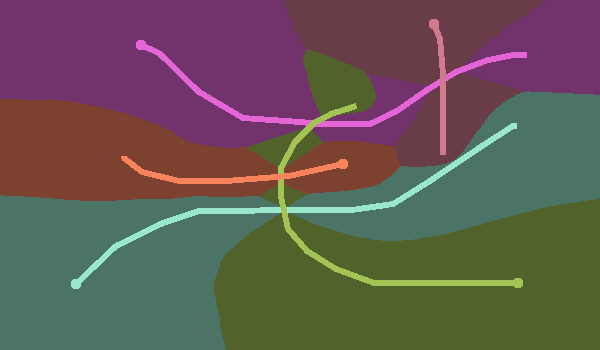
\includegraphics[scale=0.2]{sample004.png} &
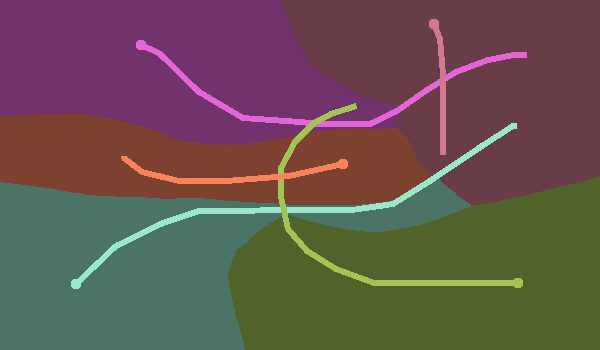
\includegraphics[scale=0.2]{sample020.png} \\
$\nu_{out} / \nu_{in} = 0.04$ & $\nu_{out} / \nu_{in} = 0.20$ \\
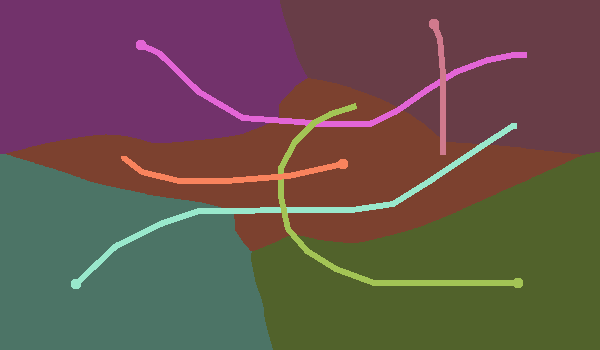
\includegraphics[scale=0.2]{sample050.png} &
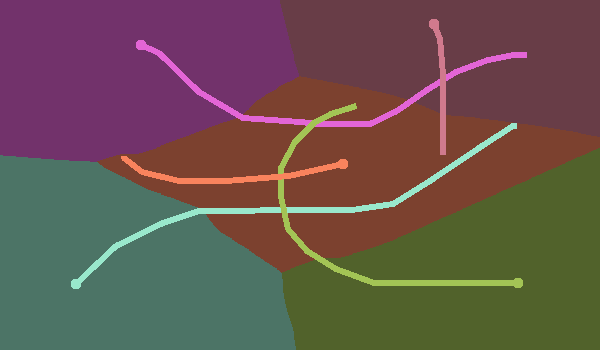
\includegraphics[scale=0.2]{sample080.png} \\
$\nu_{out} / \nu_{in} = 0.50$ & $\nu_{out} / \nu_{in} = 0.80$ \\
\multicolumn{2}{c}{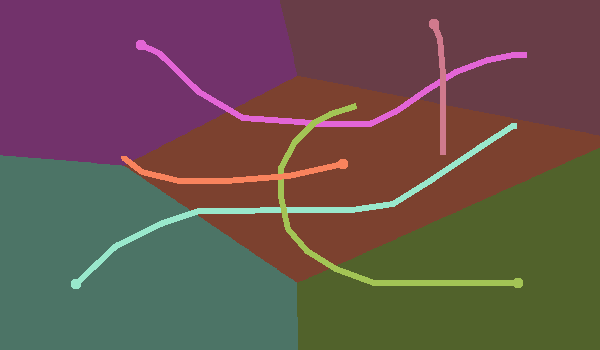
\includegraphics[scale=0.2]{sample100.png}} \\
\multicolumn{2}{c}{$\nu_{out} / \nu_{in} = 1.0$}
\end{tabular}
\end{center}
\end{figure}

\subsection{Производительность}
Измерения проивзодительности проводились на следующей вычислительной 
конфигурации: центральный процессор --- Intel\textregistered \,
Core\texttrademark \, i7-3610QM CPU, 2.30GHz;
оперативная память --- 6144MB DDR3 1600 MHz SDRAM, 6144MB; графический процессор 
--- NVIDIA® GeForce® GTX 660M. В качестве входных данных выбирались наборы ломаных
с суммарныи числом отрезков 100, 1000 и 10000 и посколько алгоритм в большей части
зависит от разрешения текстуры, а не от количества отрезков, то соответствующее 
разрешение также выбиралось различным: $1024 \times 1024$, $2048 \times 2048$, 
$4096 \times 4096$, $8192 \times 8192$. Результаты приведены на рис.~\ref{fig_perf}.

\begin{figure}
\label{fig_perf}
\begin{center}
\begin{tabular}{l l}
\begin{tikzpicture}
\begin{axis}[
    xtick = {1, 2, 3, 4},
    xticklabels={1024, 2048, 4096, 8192},
    ylabel = время работы (секунды),
    xlabel = $n$ --- размер текстуры (текселей),
    legend style={at={(0.5,1.1)},
        anchor=south,legend columns=3},
    ]
    \addplot+[sharp plot] coordinates
        {(1, 0.070) (2,0.299) (3,1.284) (4,5.470)};
    \addplot+[sharp plot] coordinates
        {(1, 0.078) (2,0.328) (3,1.399) (4,5.956)};
    \addplot+[sharp plot] coordinates
        {(1, 0.0916) (2,0.387) (3,1.616) (4,6.676)};
    \legend{100, 1000, 10000};
\end{axis}
\end{tikzpicture}
&
\begin{tikzpicture}
\begin{axis}[
    xtick = {1, 2, 3, 4},
    xticklabels={1024, 2048, 4096, 8192},
    ylabel = время работы (милисекунды),
    xlabel = $n$ --- размер текстуры (текселей),
    legend style={at={(0.5,1.1)},
        anchor=south,legend columns=3},
    ]
    \addplot+[sharp plot] coordinates
        {(1, 0.05) (2, 0.08) (3, 0.14) (4,0.26)};
    \addplot+[sharp plot] coordinates
        {(1, 1.76) (2,3.12) (3, 2.5) (4,2.56)};
    \addplot+[sharp plot] coordinates
        {(1, 36) (2,38.6) (3,36.7) (4,31)};
    \legend{100, 1000, 10000};
\end{axis}
\end{tikzpicture}
\end{tabular}
\end{center}
\caption{Время работы отдельных частей метода. Справа --- время работы 
итераций \emph{JFA+1}, слева --- время, потрачаенное на растеризацию.
разные графики соответствую разному числу отрезков-источников. }
\end{figure}

Основное узкое место алгоритма --- это большое количество обращений к памяти, 
для обработки одного элемента нужно было считать и записть приблизительно 164 байта,
поскольку при разрешении текстуры равным $n$ число итераций алгоритма составляет
$\mathrm{steps} = \lceil n \rceil + 1$, поэтому суммарное число считанных/записанных байт можно 
оценить как $\mathrm{BytesAccessed} = \mathrm{steps} * n * n * 164$. При этом 
при считывании данных об источников, как уже было замечено ранее, возможно
падение пропускной способности памяти в несколько раз меньше пиковой. Пропускная
способность алгоритма оказалось равной приблизительно 27GB/s, при том что пиковая
--- 64GB/s. Заметим, что с увеличением числа источников время выполнения \emph{JFA}
также растет, из чего можно сделать вывод о том, что при небольшом количестве источников
спасает кэш, а также тот факт, что соседние пиксели содержат часто одинаковые источники,
и при обращении к памяти данные об этом источнике можно считать лишь один раз.

Следующее узкое место алгоритма --- это вычисление оптимального пути от отрезка
до точки, потому как оно заметно сложнее, чем подобные же вычисления в \cite{jfa} и 
\cite{gvd}.

\subsection{Оценка ошибок}
Для оценки числа ошибок, на графическом процессоре был реализован наивный метод
вычисления диаграммы Вороного. Он для каждого пикселя перебирал все 
существующие источники и сохранял наилучший. Оказалось, что для текстуры 
разрешением $512x512$ относительное количество ошибок не превышает одного процента,
и быстро убывает с уменьшением шага дискретизации. Что в целом близко к
результатами, полученными в \cite{gvd}.

\section{Дальнейшие исследования}
\paragraph{Улучшение производительности.} На данный момент затруднительно полу==чить
подробную информацию об исполнении шейдеров, и сами вычислительные шейдеры появились
весьма недавно и до сих пор встречается некотороя нестабильность в их работе. В то 
время как платформа CUDA (унифицированная архитектруа вычислительных устройств, англ. 
--- Compute Unified Device Architechture) обладает богатым набором средств 
профилирования, более конкретной вычислительной моделью и является более зрелой, чем
вычислительные шейдера. В связи с чем представляется полезным перенести и настроить
алгоритм  \emph{JFA} на данной архитектуре с целью повышения производительности.

\paragraph{Сплайны.} Было бы интересно ввести источники, задаваемое в виде сплайнов,
применяемые в картографии и компьютерной графике достаточно часто. Основную сложность
здесь представляет поиск оптимального пути для сегмента сплайно (аналогично \ref{segopt}).

\paragraph{Переиспользование источников.} В данной работе повышение скорости, 
предоставляемое источниками использовалось только один раз в начале пути.
Это достаточное серьезное ограничение, которое не позволяет получить реалистичные
диаграммы Вороного на разного рода входных данных, которые не подпадают под 
сделанные в данной работе предпололожения (см.~\ref{props}). Отыскание метода,
снимающего данные ограничение широко расширит спектр допустимых входных данных.

\section{Вывод}

\pagebreak

\section{Исходный код}
\label{source}
Исходный код можно найти по следующей ссылке: 

\url{https://github.com/pschuprikov/cg-miscellaneous/tree/master/time_voronoi_diagrams}.

\begin{thebibliography}{10}
\bibitem{survey} Franz Aurenhammer. \textit{Voronoi Diagramm --- A Survey of a Fundamental Geomteric Data Structure}.
\bibitem{proced} David S. Elbert et al. \textit{Texturing and Modelling, Third Edition: A Procedural Approach}.
\bibitem{timeb} D. T. Lee, C. S. Liao, W. B. Wang. \textit{Time-Based Voronoi Diagram}.
\bibitem{distmap} Danielsson P. E. \textit{Euclidian Distance Mapping}. Computer Graphics and Image Processing 14, 227-248.
\bibitem{jfa} Guodong Rong, Tiow-Seng Tan. \textit{Jump Flooding in GPU with Applications to Voronoi Diagram and Distance Transform}. School of Computing, National University of Singapore, National University of Singapore. 
\bibitem{gvd} Zhan Yuan, Guodong Rong, Xiaohu Guo, Wenping Wang. \textit{Generalized Voronoi Diagram Computation on GPU}. The University of Hong Kong, The University of Texas at Dallas.
\end{thebibliography}
\end{document}